\documentclass[aspectratio=169]{beamer}

\usepackage[T1]{fontenc}
\usepackage[utf8]{inputenc}
\usepackage{lmodern}
\usepackage{amsmath}
\usepackage{booktabs}
\usepackage{graphicx}
\usepackage{microtype}

\usetheme{Madrid}
\usecolortheme{default}
\setbeamertemplate{navigation symbols}{}

\title[Generative models]{Generative models}
\author{Michal Pytel \and Sebastian Trojan}
\date{\today}

\begin{document}

\begin{frame}
  \titlepage
\end{frame}

\begin{frame}{Goal and Scope}
  \begin{itemize}
    \item Generate new $64\times64$ cat images from a real cat dataset.
    \item Compare three model families trained locally:
      \begin{itemize}
        \item DCGAN,
        \item variational autoencoder (VAE),
        \item denoising diffusion probabilistic model (DDPM).
      \end{itemize}
    \item Study selected hyperparameters inside each method.
    \item Evaluate with FID, sample grids, diversity diagnostics, reconstructions, and interpolation.
    \item Add an exploratory cats-and-dogs extension using the best cat-only settings.
  \end{itemize}
\end{frame}

\begin{frame}{Dataset and Preprocessing}
  \begin{columns}[T]
    \begin{column}{0.52\linewidth}
      \begin{itemize}
        \item Cat dataset: 9997 images.
        \item Mixed cats-and-dogs dataset: 25000 training images.
        \item Input images had different sizes and aspect ratios.
      \end{itemize}
    \end{column}
    \begin{column}{0.44\linewidth}
      \begin{block}{Preprocessing}
        \begin{enumerate}
          \item Convert to RGB.
          \item Centre-crop to square.
          \item Resize to $64\times64$.
          \item Random horizontal flip.
          \item Normalise to $[-1,1]$.
        \end{enumerate}
      \end{block}
    \end{column}
  \end{columns}
  \vspace{0.25cm}
  \centering
  \small
  The low resolution was chosen to make all experiments feasible on limited compute.
\end{frame}

\begin{frame}{Compared Models}
  \begin{columns}[T]
    \begin{column}{0.32\linewidth}
      \begin{block}{DCGAN}
        \begin{itemize}
          \item Latent vector $\mathbf{z}$
          \item Convolutional generator/discriminator
          \item Least-squares GAN loss
          \item Label smoothing and instance noise
        \end{itemize}
      \end{block}
    \end{column}
    \begin{column}{0.32\linewidth}
      \begin{block}{VAE}
        \begin{itemize}
          \item Encoder and decoder
          \item Gaussian latent vector
          \item Reconstruction plus KL loss
          \item Temperature-controlled sampling
        \end{itemize}
      \end{block}
    \end{column}
    \begin{column}{0.32\linewidth}
      \begin{block}{DDPM}
        \begin{itemize}
          \item U-Net denoiser
          \item Learns to predict noise
          \item Iterative reverse process
          \item Deterministic DDIM-style interpolation
        \end{itemize}
      \end{block}
    \end{column}
  \end{columns}
\end{frame}

\begin{frame}{Evaluation Protocol}
  \begin{itemize}
    \item Fr\'echet Inception Distance (FID) compares Inception feature statistics:
  \end{itemize}
  \[
    \mathrm{FID} =
    \|\mu_r - \mu_g\|_2^2 +
    \mathrm{Tr}\!\left(\Sigma_r + \Sigma_g - 2(\Sigma_r\Sigma_g)^{1/2}\right)
  \]
  \begin{itemize}
    \item DCGAN and VAE FID: 5000 generated images.
    \item DDPM FID: 2500 generated images because sampling is iterative and slower.
    \item Qualitative checks: sample grids, VAE reconstructions, and interpolation.
    \item Diversity diagnostics: pairwise RMSE and pixel standard deviation.
  \end{itemize}
\end{frame}

\begin{frame}{Hyperparameters Tested}
  \small
  \begin{tabular}{p{0.18\linewidth}p{0.72\linewidth}}
    \toprule
    Method & Main factors varied \\
    \midrule
    DCGAN &
    discriminator learning rate, generator learning rate, latent dimension, generator width,
    instance noise, label smoothing, minibatch-standard-deviation feature \\
    VAE &
    KL strength, prior-matching variant, latent dimension, decoder refinement,
    multiscale reconstruction loss, sampling temperature \\
    DDPM &
    U-Net width, noise schedule, learning rate, dropout, number of diffusion timesteps \\
    \bottomrule
  \end{tabular}

  \vspace{0.35cm}
  \begin{itemize}
    \item Each model family was compared internally by changing one main factor at a time.
    \item All variants were trained for 300 epochs.
    \item FID was interpreted together with generated grids and diversity diagnostics.
  \end{itemize}
\end{frame}

\begin{frame}{Best Hyperparameter Results}
  \scriptsize
  \begin{columns}[T]
    \begin{column}{0.32\linewidth}
      \centering
      \textbf{DCGAN}\\[0.1cm]
      \begin{tabular}{lr}
        \toprule
        Variant & FID \\
        \midrule
        D LR $10^{-4}$ & \textbf{143.79} \\
        G width 96 & 153.95 \\
        No noise & 155.60 \\
        Baseline & 161.62 \\
        \bottomrule
      \end{tabular}
    \end{column}
    \begin{column}{0.32\linewidth}
      \centering
      \textbf{VAE}\\[0.1cm]
      \begin{tabular}{lrr}
        \toprule
        Variant & Temp. & FID \\
        \midrule
        $\beta=0.5$ & 0.65 & \textbf{176.68} \\
        Prior & 0.50 & 189.33 \\
        $\beta=0.25$ & 0.50 & 191.54 \\
        Extra decoder & 0.50 & 193.75 \\
        \bottomrule
      \end{tabular}
    \end{column}
    \begin{column}{0.32\linewidth}
      \centering
      \textbf{DDPM}\\[0.1cm]
      \begin{tabular}{lr}
        \toprule
        Variant & FID \\
        \midrule
        Width 96 & \textbf{48.00} \\
        Baseline & 48.90 \\
        Cosine & 64.18 \\
        LR $10^{-4}$ & 70.61 \\
        \bottomrule
      \end{tabular}
    \end{column}
  \end{columns}

  \vspace{0.35cm}
  \small
  The best model inside each family was used for the final comparison.
\end{frame}

\begin{frame}{VAE Temperature Results}
  \begin{columns}[T]
    \begin{column}{0.46\linewidth}
      \centering
      \small
      \begin{tabular}{lrr}
        \toprule
        Temp. & Mean FID $\pm$ std. & Best FID \\
        \midrule
        0.50 & \textbf{209.25 $\pm$ 24.10} & 188.23 \\
        0.65 & 209.89 $\pm$ 20.78 & \textbf{176.68} \\
        0.80 & 230.99 $\pm$ 14.74 & 199.93 \\
        \bottomrule
      \end{tabular}
      \vspace{0.25cm}
      \begin{itemize}
        \item 0.50 keeps latent samples closer to the prior centre: smoother but less varied.
        \item 0.65 gives a moderate amount of variation while keeping more cat-like structure.
        \item 0.80 explores farther latent regions, which increases malformed textures and anatomy.
      \end{itemize}
    \end{column}
    \begin{column}{0.50\linewidth}
      \centering
      \scriptsize
      \begin{minipage}{0.32\linewidth}
        \centering
        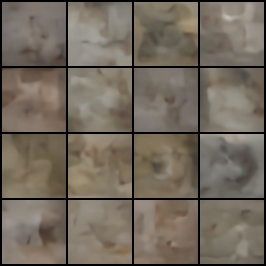
\includegraphics[width=\linewidth]{report_figures/vae_temperature_050.png}\\
        Temp. 0.50
      \end{minipage}
      \begin{minipage}{0.32\linewidth}
        \centering
        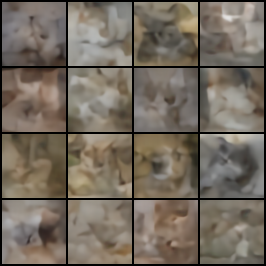
\includegraphics[width=\linewidth]{report_figures/vae_temperature_065.png}\\
        Temp. 0.65
      \end{minipage}
      \begin{minipage}{0.32\linewidth}
        \centering
        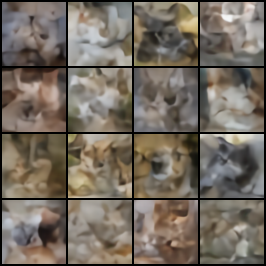
\includegraphics[width=\linewidth]{report_figures/vae_temperature_080.png}\\
        Temp. 0.80
      \end{minipage}
      \vspace{0.15cm}

      Same seed and $\beta=0.5$ model.
    \end{column}
  \end{columns}
\end{frame}

\begin{frame}{VAE Reconstructions}
  \centering
  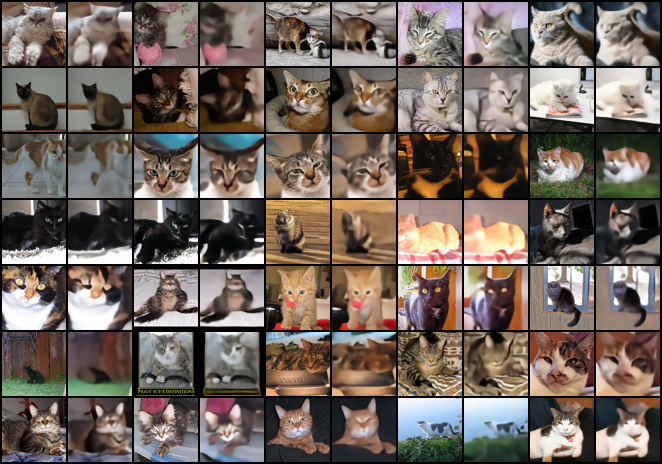
\includegraphics[width=0.92\linewidth,height=0.70\textheight,keepaspectratio]{report_figures/vae_reconstructions.png}
  \vspace{0.15cm}

  \small
  Reconstructions preserve pose and colour better than random samples, but texture and edges are smoothed.
\end{frame}

\begin{frame}{Final Quantitative Comparison}
  \centering
  \small
  \begin{tabular}{lrrr}
    \toprule
    Method & FID & Diversity RMSE & Pixel std. \\
    \midrule
    DCGAN & 143.79 & 0.3682 & 0.2644 \\
    VAE & 176.68 & 0.1351 & 0.0966 \\
    DDPM & \textbf{48.00} & \textbf{0.4179} & \textbf{0.3084} \\
    \bottomrule
  \end{tabular}

  \vspace{0.55cm}
  \begin{itemize}
    \item DDPM had the strongest FID and diversity diagnostics.
    \item DCGAN produced sharper images than VAE, but more distorted outputs.
    \item VAE was stable and reconstructed real cats well, but random samples were blurry.
  \end{itemize}
\end{frame}

\begin{frame}{Qualitative Cat-Only Results}
  \centering
  \begin{columns}[T]
    \begin{column}{0.32\linewidth}
      \centering
      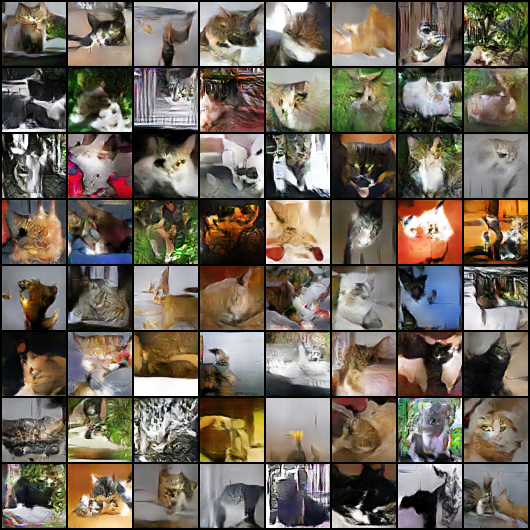
\includegraphics[width=\linewidth]{report_figures/dcgan_samples.png}
      \small DCGAN
    \end{column}
    \begin{column}{0.32\linewidth}
      \centering
      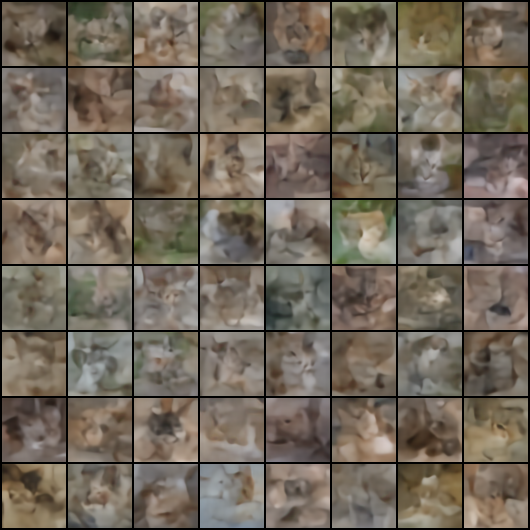
\includegraphics[width=\linewidth]{report_figures/vae_samples.png}
      \small VAE
    \end{column}
    \begin{column}{0.32\linewidth}
      \centering
      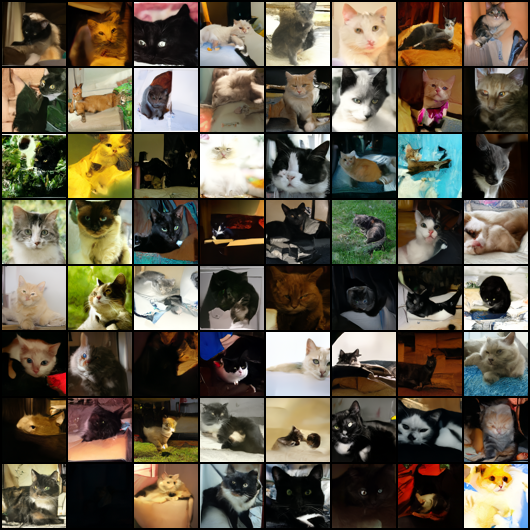
\includegraphics[width=\linewidth]{report_figures/ddpm_samples.png}
      \small DDPM
    \end{column}
  \end{columns}
  \vspace{0.3cm}
  \small
  DDPM produced the most recognisable and varied cat samples; VAE samples were the smoothest.
\end{frame}

\begin{frame}{Interpolation Comparison}
  \centering
  \scriptsize
  \begin{tabular}{rl}
    DCGAN &
    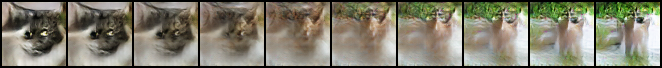
\includegraphics[width=0.78\textwidth,height=0.17\textheight,keepaspectratio]{report_figures/dcgan_interpolation.png} \\
    VAE &
    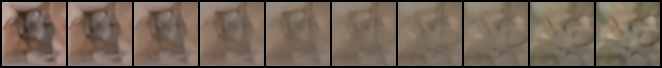
\includegraphics[width=0.78\textwidth,height=0.17\textheight,keepaspectratio]{report_figures/vae_interpolation.png} \\
    DDPM &
    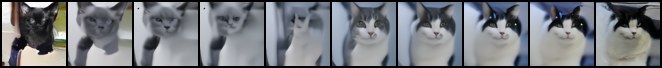
\includegraphics[width=0.78\textwidth,height=0.17\textheight,keepaspectratio]{report_figures/ddpm_interpolation.png} \\
  \end{tabular}

  \vspace{0.25cm}
  \small
  Each row shows 10 points: two endpoints and eight linear interpolations.
  DDPM gave the smoothest semantic transition; VAE was smooth but blurry, and DCGAN was less stable in the middle samples.
\end{frame}

\begin{frame}{Mode Collapse and Diversity}
  \begin{itemize}
    \item Mode collapse was checked with sample grids and simple pixel-space diversity diagnostics.
    \item Final diversity RMSE values:
      \begin{itemize}
        \item DCGAN: 0.3682,
        \item VAE: 0.1351,
        \item DDPM: 0.4179.
      \end{itemize}
    \item DCGAN did not collapse to one image type, but repeated textures and malformed samples appeared.
    \item DDPM showed the highest measured diversity.
  \end{itemize}
\end{frame}

\begin{frame}{Cats-and-Dogs Extension: FID}
  \centering
  \small
  \begin{tabular}{lr}
    \toprule
    Method & FID \\
    \midrule
    DCGAN & 131.02 \\
    VAE & 246.27 \\
    DDPM & \textbf{74.23} \\
    \bottomrule
  \end{tabular}

  \vspace{0.45cm}
  \begin{itemize}
    \item Same best cat-only settings were reused.
    \item Models were unconditional: no class label was provided.
    \item FID was computed against the mixed cats-and-dogs distribution.
    \item The metric does not prove clean class separation between cats and dogs.
  \end{itemize}
\end{frame}

\begin{frame}{Cats-and-Dogs Extension: Samples}
  \centering
  \begin{columns}[T]
    \begin{column}{0.32\linewidth}
      \centering
      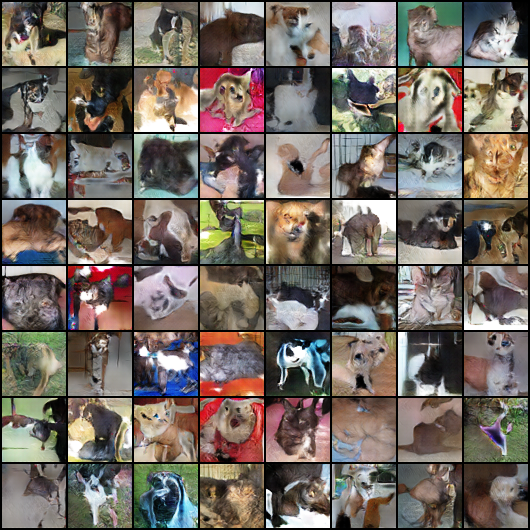
\includegraphics[width=\linewidth,height=0.62\textheight,keepaspectratio]{report_figures/catdog_dcgan_samples.png}\\
      \small DCGAN
    \end{column}
    \begin{column}{0.32\linewidth}
      \centering
      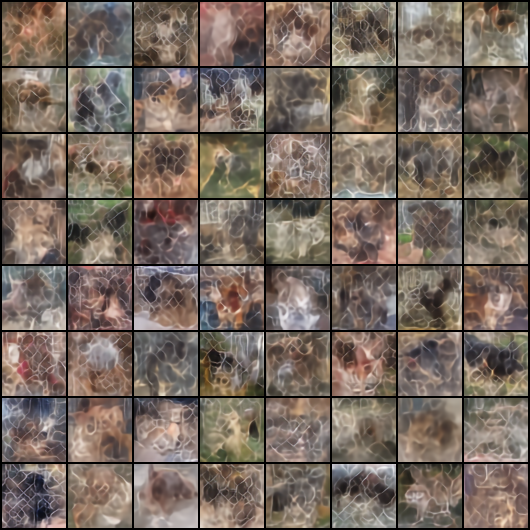
\includegraphics[width=\linewidth,height=0.62\textheight,keepaspectratio]{report_figures/catdog_vae_samples.png}\\
      \small VAE
    \end{column}
    \begin{column}{0.32\linewidth}
      \centering
      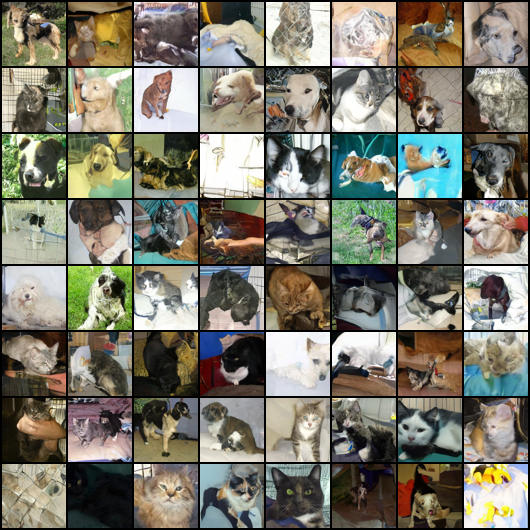
\includegraphics[width=\linewidth,height=0.62\textheight,keepaspectratio]{report_figures/catdog_ddpm_samples.png}\\
      \small DDPM
    \end{column}
  \end{columns}

  \vspace{0.2cm}
  \small
  Mixed-data generations include cat-like, dog-like, and ambiguous animal samples.
\end{frame}

\begin{frame}{Conclusions}
  \begin{itemize}
    \item The wider DDPM was the strongest model overall.
    \item DCGAN was a useful lightweight alternative, but less stable.
    \item VAE reconstructed real images well, but random samples from the prior were weak.
    \item FID alone was not enough: qualitative grids and diversity checks were necessary.
    \item The mixed cats-and-dogs experiment confirmed that unconditional generation can create ambiguous samples when classes are combined.
  \end{itemize}

  \vspace{0.4cm}
  \begin{block}{Main takeaway}
    For this limited-compute setup, DDPM gave the best balance of quality, diversity, and interpolation behaviour.
  \end{block}
\end{frame}

\end{document}
